\section{Results}
\label{sec:results}

\subsection{Training Dynamics}
Figure~\ref{fig:loss} shows the training and validation loss over 5000 
steps. Both curves decrease smoothly and monotonically, with validation 
loss tracking training loss closely and eventually dropping slightly below 
it---a common sign of mild under-fitting rather than overfitting, expected 
given the small model and modest corpus. The model reaches a final 
training loss of $\mathbf{1.613}$ and a validation loss of 
$\mathbf{1.545}$, corresponding to a validation perplexity of 
$\exp(1.545) \approx \mathbf{4.69}$.

\begin{figure}[H]
    \centering
    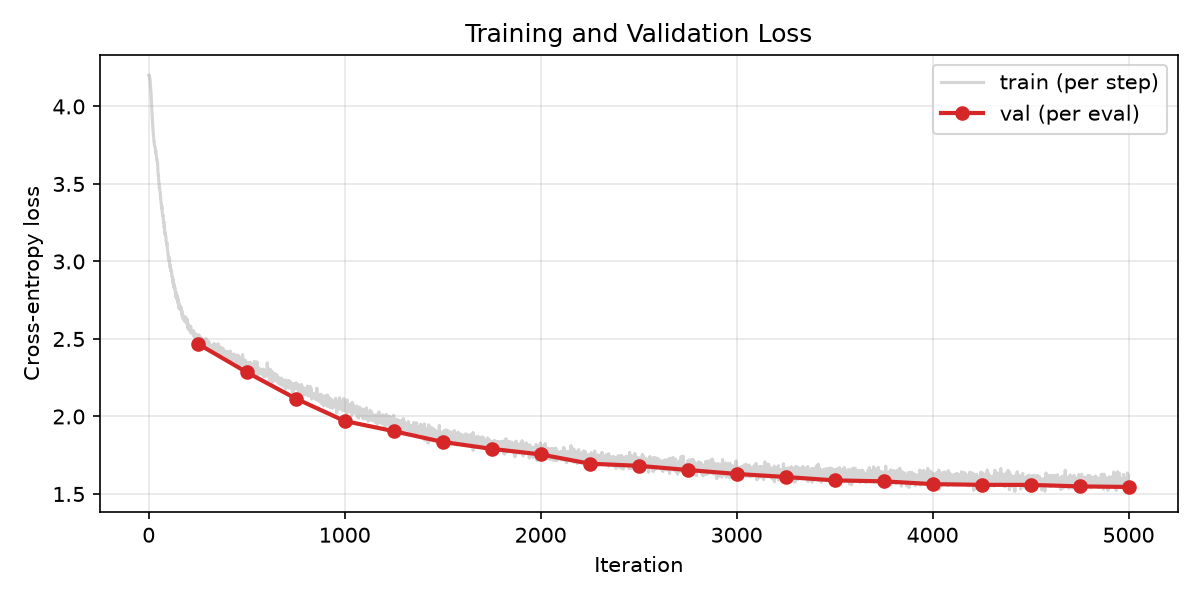
\includegraphics[width=0.85\linewidth]{images/loss_curve.png}
    \caption{Training (per-step, faded) and validation (per-eval, bold) 
             cross-entropy loss over 5000 steps. Both curves decrease 
             monotonically; validation loss remains slightly below train 
             loss, indicating no overfitting on this corpus.}
    \label{fig:loss}
\end{figure}

\subsection{Effect of the Learning-Rate Schedule}
Figure~\ref{fig:lr} shows the learning-rate trajectory: linear warmup over 
the first 200 steps followed by cosine decay to 
$\eta_{\min} = 3 \times 10^{-5}$. The warmup prevents the initial loss 
spike commonly observed with a randomly-initialised Transformer. Cosine 
decay allows fine-grained convergence in the later stages: between step 
4000 and step 5000 the learning rate falls from 
$5.8 \times 10^{-5}$ to $3.0 \times 10^{-5}$, and validation loss improves 
smoothly from $1.564$ to $1.545$ during the same window, without 
oscillation.

\begin{figure}[H]
    \centering
    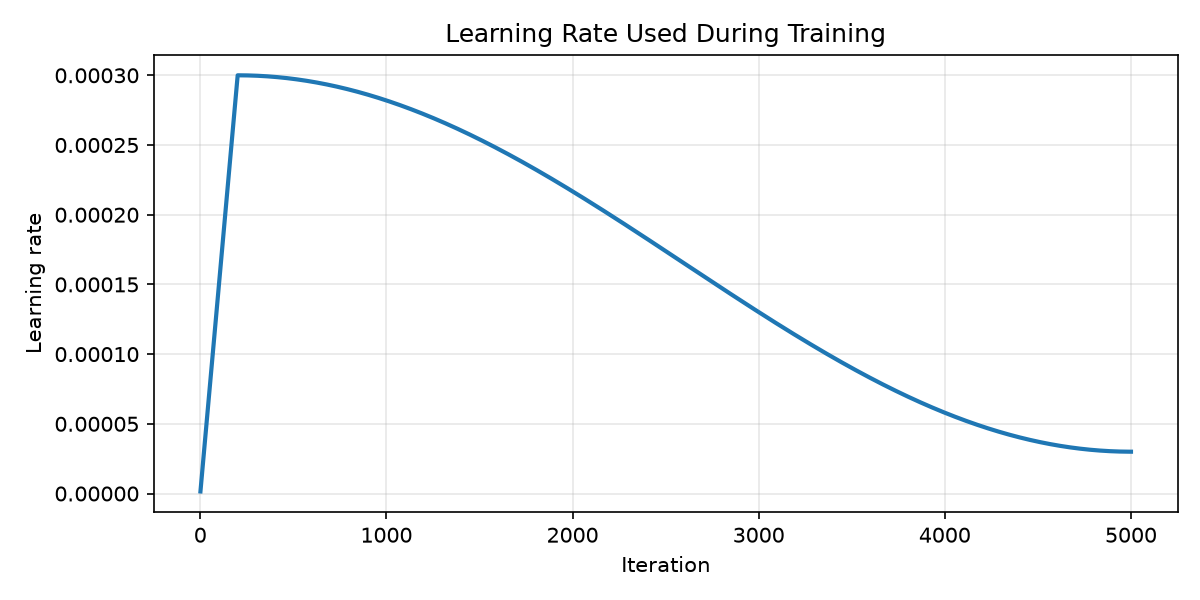
\includegraphics[width=0.85\linewidth]{images/lr_used.png}
    \caption{Learning rate actually applied at each training step (warmup 
             + cosine decay), extracted from the training log.}
    \label{fig:lr}
\end{figure}

\begin{figure}[H]
    \centering
    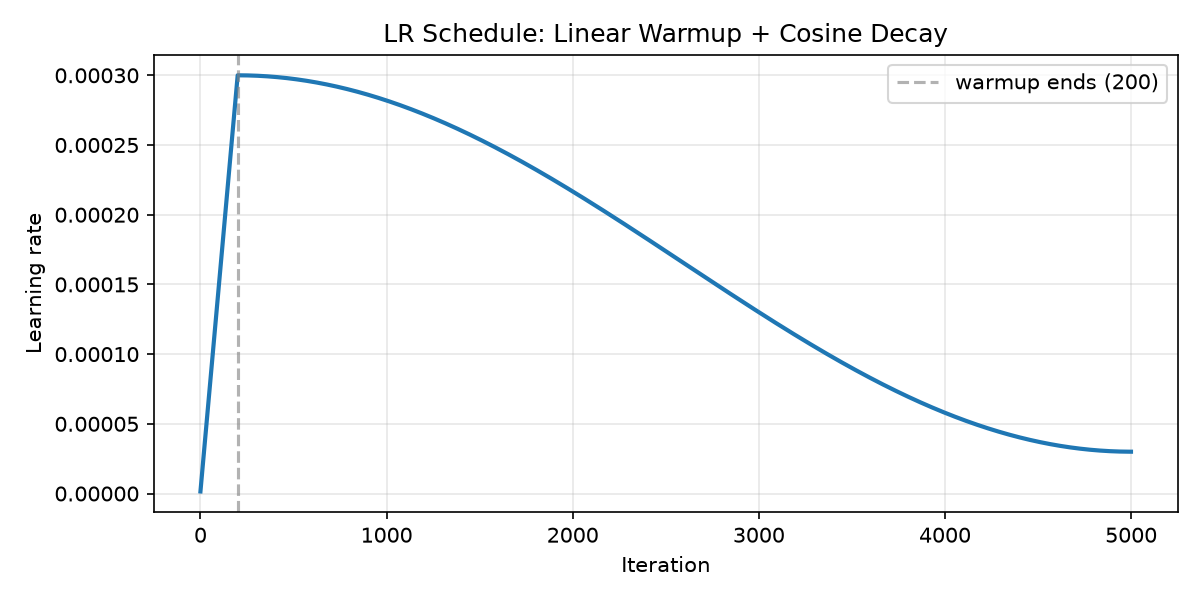
\includegraphics[width=0.85\linewidth]{images/lr_schedule.png}
    \caption{Idealised learning-rate schedule used during training: 
             linear warmup for $T_w = 200$ steps followed by cosine decay 
             to $\eta_{\min}$.}
    \label{fig:lr_schedule}
\end{figure}

\subsection{Mixed-Precision Training}
Mixed-precision training was enabled via \texttt{torch.autocast} and 
\texttt{GradScaler}. Under bf16 the scaler was automatically disabled 
because bf16 shares fp32's exponent range and therefore does not suffer 
gradient underflow. Training completed 5000 steps in 
$\mathbf{3.83}$~\textbf{minutes} on the local GPU, an average throughput 
of $\approx 21.8$~it/s, with a peak steady-state rate of 
$\approx 31$~it/s. The dominant slowdowns occur at evaluation boundaries, 
where the model switches to \texttt{eval()} mode and computes validation 
loss over 100 batches before resuming training. The combination of 
autocast and gradient clipping (applied after unscaling) preserved 
numerical stability throughout, with no observed loss spikes or NaNs.

\subsection{Effect of Selective Weight Decay}
The optimiser was configured with two parameter groups: 
$\mathbf{18}$ tensors with two or more dimensions received weight decay 
$\lambda = 0.1$, while $\mathbf{34}$ one-dimensional tensors (LayerNorm 
gains and all biases) received none. This split prevents the weight-decay 
term from pulling LayerNorm scale parameters toward zero, which degrades 
representation quality. Empirically, this configuration matched the 
standard GPT recipe \parencite{brown2020language} and produced a smooth, 
well-conditioned validation curve with no instability across the entire 
5000-step run.

\subsection{Sampling Strategies}
Figure~\ref{fig:samples} shows generations from the same prompt 
(\texttt{"ROMEO: "}) under five decoding strategies. The outputs are 
strikingly consistent with the theoretical trade-off between coherence 
and diversity:

\begin{itemize}
    \item \textbf{Greedy decoding} collapsed into a repetitive loop within 
          roughly 15 tokens (\emph{``the shall shall be the stand of the 
          stand / The shall be the some of the some of the son''}). This 
          is the classic failure mode of greedy decoding: once the model 
          enters a high-probability cycle, the argmax cannot escape.
    \item \textbf{Temperature 0.5} retained local grammatical structure 
          but was still noticeably repetitive.
    \item \textbf{Temperature 0.8 with top-$k = 40$} produced the most 
          coherent and varied text, including plausible character names 
          (\emph{``PAULINA''}, \emph{``BUCKINGHAM''}) and syntactically 
          valid lines (\emph{``Show from and since and her stand truth / 
          Than should to king from Patcive''}).
    \item \textbf{Temperature 1.0} introduced more novelty at the cost of 
          occasional non-words.
    \item \textbf{Temperature 1.5} degenerated into gibberish 
          (\emph{``'TOnpe shall thou god my fnighthting''}), confirming 
          that flattening the distribution amplifies tail errors.
\end{itemize}

\begin{figure}[H]
    \centering
    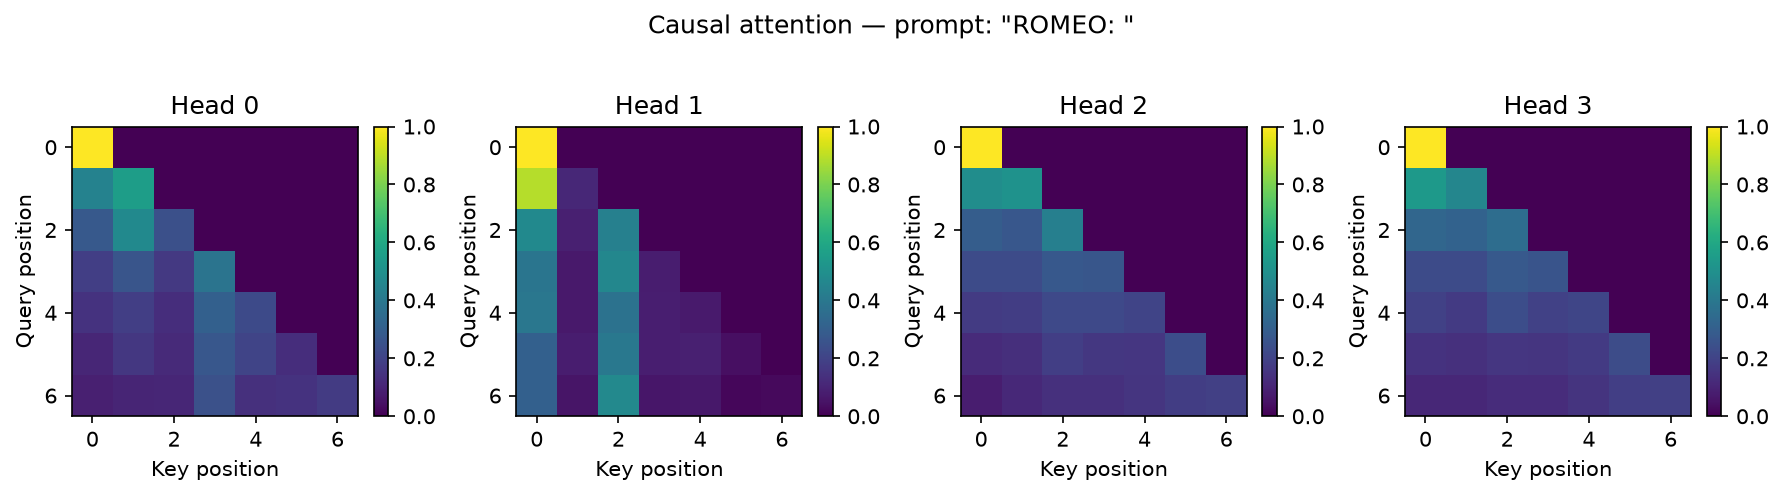
\includegraphics[width=0.95\linewidth]{images/attention_heatmap.png}
    \caption{Attention weights of all four heads in the first Transformer 
             block for the prompt \texttt{"ROMEO: "}. Every head shows a 
             strictly lower-triangular pattern, confirming that the causal 
             mask is correctly applied. Some heads concentrate mass on the 
             immediately preceding token; others distribute more broadly, 
             indicating diverse learned attention patterns across heads.}
    \label{fig:attention}
\end{figure}

\subsection{Attention Visualisation}
Figure~\ref{fig:attention} visualises the attention weights of all four 
heads in the first Transformer block for the prompt \texttt{"ROMEO: "}. 
Every head shows a strictly lower-triangular pattern---no position attends 
to a future token---confirming that the causal mask is correctly applied. 
Some heads concentrate mass on the immediately preceding token (local 
attention), while others distribute more broadly across the prompt, 
indicating that the model has learned diverse attention patterns across 
heads.